\chapter{系统体系结构}
根据已选用的软件、硬件以及网络环境构造系统的整体框架,划分系统模块,并对系统内各个模块之间的关系进行定义。确定已定义的对象及其组件在系统内如何传输、通信。如果本系统是用户最终投入使用系统的一个子集或是将要使用现有的一些其他相关系统,那么在此应对它们各自的功能和相互之间的关系给予具体的描述。

\section{处理流程}
\subsection{总体流程}
[可通过图形的方式表示系统体系结构,以下给了一个案例写法供参考。]

\begin{figure}[htbp!]
    \centering
    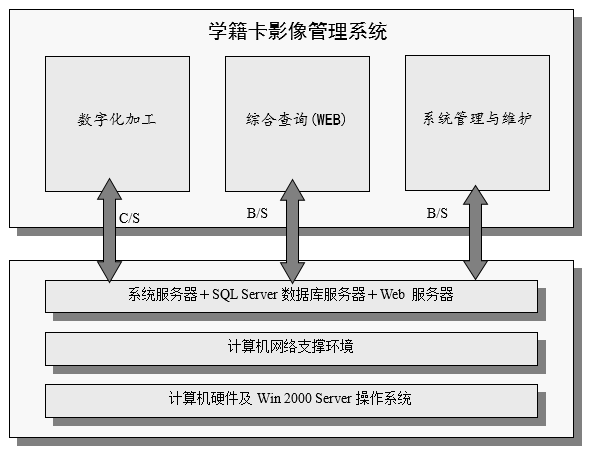
\includegraphics[width=0.8\linewidth]{fig-example.png}
    \caption{体系结构图}
    \label{fig:my_label}
\end{figure}
